\chapter{Fixed-Parameter Tractability on Graphs}

Most of the deep graph problems worth caring about are NP-hard: vertex cover, feedback vertex set, longest path, clique, dominating set. The classical theory of NP-completeness paints them all with the same brush --- ``no polynomial algorithm unless P${}={}$NP'' --- and then walks away. That verdict is correct but coarse. It measures everything against a single yardstick, the input size $n$, and declares defeat the moment the running time refuses to be polynomial in $n$.

Parameterized complexity refuses to accept such a flat picture. It asks a sharper question: \emph{where} does the exponential blow-up really live? For vertex cover, you usually do not want a cover of arbitrary size; you want to know whether one of size at most $k$ exists, and in practice $k$ is small --- a network with a few critical routers, a conflict graph with a handful of irreconcilable pairs. If we could push the entire combinatorial explosion onto $k$ and keep the dependence on $n$ polynomial, then for small $k$ the problem would be entirely tractable, NP-hardness notwithstanding. That is the whole idea: a second dimension, the \emph{parameter} $k$, soaks up the hardness.

This chapter develops the toolkit. We will see four techniques that each turn an exponential search into something of the form $f(k)\cdot\poly(n)$: bounded search trees, kernelization, iterative compression, and color coding. Each one is a small idea executed with care, and each one is best learned by running it by hand on a graph small enough to hold in your head. We close with the W-hierarchy, the parameterized world's answer to ``but what about the problems that resist all four techniques?''

\chapterline

\section{The parameterized lens}

Fix a problem and a way to read a second number $k$ off each instance. Formally a \emph{parameterized problem} is a language $L \subseteq \Sigma^* \times \N$; an instance is a pair $(x,k)$ where $x$ is the usual input (a graph, say) of size $n=\abs{x}$ and $k$ is the parameter.

\begin{definition}[Fixed-parameter tractable]\label{ch25:def-fpt}
A parameterized problem is \emph{fixed-parameter tractable} (FPT) if there is an algorithm deciding $(x,k)\in L$ in time
\[
  f(k)\cdot \abs{x}^{c}
\]
for some computable function $f$ and a constant $c$ independent of both $n$ and $k$. The class of all such problems is denoted FPT.
\end{definition}

The function $f$ is allowed to be monstrous --- $2^k$, $k!$, $2^{2^k}$ --- but it touches only the parameter. The dependence on the input size is a fixed polynomial. Contrast this with the obvious brute force.

\begin{definition}[Slice-wise polynomial]\label{ch25:def-xp}
A problem is in XP if it can be solved in time $f(k)\cdot \abs{x}^{g(k)}$ for computable $f,g$. Equivalently, for every fixed $k$ there is a polynomial-time algorithm, but the degree of the polynomial is allowed to grow with $k$.
\end{definition}

\begin{intuitionbox}
The difference between FPT and XP is the difference between $2^k\cdot n$ and $n^k$. Both are ``polynomial for fixed $k$,'' but only one is usable. Take $n=10^6$ and $k=20$. The FPT bound $2^{20}\cdot 10^6 \approx 10^{12}$ is a long afternoon. The XP bound $n^k = (10^6)^{20} = 10^{120}$ is more operations than there are atoms in the observable universe, many times over. FPT moves the exponent off $n$; XP leaves it sitting on $n$. The exponent on the input size is the whole ballgame.
\end{intuitionbox}

\begin{focusbox}
A handful of facts we lean on throughout.
\begin{itemize}
  \item FPT $\subseteq$ XP, and the inclusion is strict (there are problems solvable in $n^{f(k)}$ time but provably not in $f(k)\cdot n^{O(1)}$).
  \item Brute-force ``try all $\binom{n}{k}$ subsets'' is the canonical XP algorithm: $\Oh(n^k)$. The art is to replace it by $f(k)\cdot n^{O(1)}$.
  \item A problem is FPT \emph{if and only if} it admits a kernel (Theorem~\ref{ch25:thm-kernel-iff}). This equivalence is the backbone of the field.
  \item The choice of parameter matters enormously. Vertex cover parameterized by solution size is FPT; parameterized by treewidth it is also FPT; clique parameterized by solution size is believed \emph{not} to be FPT. Same graphs, different knob.
\end{itemize}
\end{focusbox}

\begin{historybox}
Parameterized complexity was founded in the late 1980s and 1990s by Rod Downey and
Michael Fellows. In practical applications ranging from VLSI circuit design to computational
biology and compiler register allocation, engineers repeatedly faced NP-hard problems where
a critical budget or threshold parameter $k$ was small ($k \le 15$), while the graph size $n$
was massive ($n \ge 10^6$). Classical Cook--Karp NP-completeness declared all these problems
flatly intractable, offering no guidance on why some small-parameter instances were easily
solved while others resisted all computation.

A glaring paradox in Karp's original 1972 reductions fueled the controversy: Vertex Cover
and Independent Set are polynomial-time equivalent via the trivial complement map ($S$ is an
independent set if and only if $V \setminus S$ is a vertex cover). Yet Vertex Cover possessed
an $\Oh(2^k n)$ bounded search tree, while Independent Set seemed to require $\Oh(n^k)$
brute-force search. Early researchers spent years trying to adapt Vertex Cover branching
and kernelization rules to Independent Set and Clique, but every attempt failed.

Downey and Fellows unlocked the puzzle by proving that standard polynomial-time Karp reductions
do not preserve parameter size: a cover of size $k$ maps to an independent set of size $n - k$,
turning a small parameter into a massive one! To separate these behaviors, they invented
\emph{parameterized reductions} (requiring the new parameter $k' \le g(k)$) and erected the
W-hierarchy ($W[1], W[2], \dots$). By proving that $k$-Clique is $W[1]$-hard, they provided the
first mathematical proof that Vertex Cover and Independent Set belong to fundamentally
distinct complexity classes under parameterization.
\end{historybox}

\section{A graph to carry through the chapter}

We will keep returning to one small graph. Meet $\Gph$: seven vertices, drawn so you can see its structure.

\begin{figure}[H]
\centering
\begin{tikzpicture}[every node/.style={circle,draw,fill=blue!8,minimum size=8mm,inner sep=1pt,font=\small},
  thick,>=Stealth]
  \node (a) at (0,2)   {a};
  \node (b) at (2,3)   {b};
  \node (c) at (4,2.4) {c};
  \node (d) at (2,1)   {d};
  \node (e) at (4,0.4) {e};
  \node (f) at (6,1.6) {f};
  \node (g) at (6,3)   {g};
  \draw (a)--(b);
  \draw (a)--(d);
  \draw (b)--(c);
  \draw (b)--(d);
  \draw (c)--(d);
  \draw (c)--(e);
  \draw (c)--(g);
  \draw (d)--(e);
  \draw (e)--(f);
  \draw (f)--(g);
\end{tikzpicture}
\caption{Running example $\Gph=(V,E)$ with $V=\{a,b,c,d,e,f,g\}$ and ten edges. The triangles $a\,b\,d$, $b\,c\,d$, $c\,d\,e$ and the $4$-cycle $c\,e\,f\,g$ overlap, which makes it a useful test bed for both vertex cover and feedback vertex set.}
\label{ch25:fig-running}
\end{figure}

\begin{labbox}
Before the algorithms arrive, find a vertex cover of $\Gph$ by hand --- a set of vertices touching every edge. Try $\{b,c,d,e\}$: edge $f\,g$ is left uncovered, so no. Now hunt for size $4$. Test $\{b,c,d,f\}$ against all ten edges: $ab$ (b), $ad$ (d), $bc$ (b), $bd$ (b), $cd$ (c), $ce$ (c), $cg$ (c), $de$ (d), $ef$ (f), $fg$ (f). All covered. So $\{b,c,d,f\}$ is a cover of size $4$. Keep this number $4$ in mind.
\end{labbox}

\section{Bounded search trees: vertex cover in \texorpdfstring{$\Oh(2^k(n+m))$}{O(2^k(n+m))}}

The first technique is the most elementary and the most broadly useful. The idea: make a \emph{branching} decision that is forced to be small (at most a constant number of options) and that decreases the parameter by at least one on every branch. The recursion then has bounded depth $k$ and bounded fan-out, so the tree of recursive calls has size $f(k)$, and each node does polynomial work.

\subsection{The branching rule}

\textsc{Vertex Cover}: given $\Gph=(V,E)$ and an integer $k$, is there a set $S\subseteq V$ with $\abs{S}\le k$ covering every edge?

Pick any edge $\{u,v\}$ that is still uncovered. Any vertex cover must contain $u$ or $v$ --- otherwise that edge is left naked. That is the entire insight, and it is a binary branch:
\[
  \text{either } u\in S \quad\text{or}\quad v\in S.
\]
In the first branch we put $u$ into the cover, delete $u$ (and all its incident edges), and recurse with budget $k-1$. In the second we do the same with $v$. Each branch spends one unit of budget. After at most $k$ levels we either run out of edges (success) or run out of budget (failure on this path).

\begin{algorithm}[H]
\caption{\textsc{VC-Branch}$(\Gph,k)$ --- bounded search tree for vertex cover}
\label{ch25:alg-vcbranch}
\DontPrintSemicolon
\KwIn{graph $\Gph=(V,E)$, budget $k\ge 0$}
\KwOut{a vertex cover of size $\le k$, or \textsc{None}}
\If{$E=\emptyset$}{ \Return $\emptyset$ \tcp*{all edges covered} }
\If{$k=0$}{ \Return \textsc{None} \tcp*{out of budget but edges remain} }
pick any edge $\{u,v\}\in E$\;
$S_u \gets \textsc{VC-Branch}(\Gph - u,\; k-1)$\;
\lIf{$S_u \neq \textsc{None}$}{ \Return $S_u \cup \{u\}$ }
$S_v \gets \textsc{VC-Branch}(\Gph - v,\; k-1)$\;
\lIf{$S_v \neq \textsc{None}$}{ \Return $S_v \cup \{v\}$ }
\Return \textsc{None}\;
\end{algorithm}

Here $\Gph - u$ denotes $\Gph$ with vertex $u$ and its incident edges removed.

\begin{whybox}
\textbf{Correctness.} We argue \textsc{VC-Branch}$(\Gph,k)$ returns a cover of size $\le k$ iff one exists. The base cases are immediate: no edges means the empty set covers everything; no budget but a surviving edge means failure on this branch. For the inductive step, fix an edge $\{u,v\}$. Every vertex cover contains $u$ or $v$. If a cover $S^\star$ of size $\le k$ exists and $u\in S^\star$, then $S^\star\setminus\{u\}$ is a cover of $\Gph-u$ of size $\le k-1$, which the recursion on the $u$-branch finds by induction; symmetrically if $v\in S^\star$. Conversely any set the algorithm returns is, by construction, a union of branch vertices that together hit every deleted edge, hence a genuine cover. The two branches are exhaustive because the alternatives ``$u\in S$'' and ``$v\in S$'' cover all possibilities (they may overlap; that is fine, we only need completeness).
\end{whybox}

\begin{whybox}
\textbf{Complexity.} Let $T(k)$ be the number of leaves of the search tree. The recurrence is $T(k) = 2\,T(k-1)$ with $T(0)=1$, so $T(k)\le 2^k$. The tree has $\Oh(2^k)$ nodes. At each node we find an uncovered edge and delete a vertex, $\Oh(n+m)$ work with adjacency lists. Total:
\[
  \Oh\!\big(2^k (n+m)\big).
\]
For $k=20$ on a million-edge graph this is about $10^{12}$ basic steps --- feasible. The naive $\binom{n}{k}$ enumeration would be $\binom{10^6}{20}\approx 10^{100}$. The branching has moved the exponent entirely onto $k$.
\end{whybox}

\subsection{Trace on the running graph}

Run \textsc{VC-Branch}$(\Gph,4)$ on Figure~\ref{ch25:fig-running}. Suppose the edge picker always returns the lexicographically first uncovered edge.

\begin{labbox}
\textbf{Step by step.} The algorithm explores the first endpoint of each chosen edge first, so we follow that branch and watch it succeed.
\begin{itemize}
  \item First edge: $ab$. Take the $a$-branch: delete $a$, budget $3$. Edges left: $bc,bd,cd,ce,cg,de,ef,fg$ (the edges $ab,ad$ vanished with $a$).
  \item First edge now $bc$. Take the $c$-branch: delete $c$, budget $2$. Edges left: $bd,de,ef,fg$ (the edges $bc,cd,ce,cg$ vanished with $c$).
  \item First edge $bd$. Take the $d$-branch: delete $d$, budget $1$. Edges left: $ef,fg$ (the edges $bd,de$ vanished with $d$).
  \item First edge $ef$. Take the $f$-branch: delete $f$, budget $0$. Edges left: $\emptyset$. Success with $\{a,c,d,f\}$, a size-$4$ cover.
\end{itemize}
The search tree visits at most $2^4=16$ leaves; the winning path is one root-to-leaf walk of length $4$. The algorithm returns the first size-$4$ cover it reaches; here that is $\{a,c,d,f\}$ rather than the $\{b,c,d,f\}$ we found by hand earlier, but both are valid covers of size $4$.
\end{labbox}

\begin{figure}[H]
\centering
\begin{tikzpicture}[every node/.style={font=\footnotesize},level distance=12mm,
  level 1/.style={sibling distance=46mm},
  level 2/.style={sibling distance=23mm},
  edge from parent/.style={draw,->,>=Stealth,thick}]
\node[draw,rounded corners,fill=blue!6] {$k{=}4$, edge $ab$}
  child {node[draw,rounded corners,fill=green!8] {$a\in S$, $k{=}3$, edge $bc$}
    child {node[draw,rounded corners,fill=green!6] {$b\in S$, $k{=}2$}}
    child {node[draw,rounded corners,fill=green!10] {$c\in S$, $k{=}2$ $\to\cdots\to\{a,c,d,f\}$}}
  }
  child {node[draw,rounded corners,fill=red!6] {$b\in S$, $k{=}3$}
    child {node[draw,rounded corners,fill=red!4] {$\cdots$}}
    child {node[draw,rounded corners,fill=red!4] {$\cdots$}}
  };
\end{tikzpicture}
\caption{Top of the bounded search tree for \textsc{VC-Branch}$(\Gph,4)$. Each branch fixes one endpoint of an uncovered edge and spends one unit of budget; depth is at most $k=4$, fan-out is $2$, so at most $2^4$ leaves. The algorithm explores the $a$-branch first; the green path reaches the cover $\{a,c,d,f\}$, so the $b$-branch is never visited.}
\label{ch25:fig-searchtree}
\end{figure}

\begin{trapbox}
A tempting ``optimization'' is to branch greedily on a maximum-degree vertex: ``either the high-degree vertex $u$ is in the cover, or it is not.'' But the second branch ``$u\notin S$'' is \emph{not} free: it forces \emph{all} neighbors of $u$ into the cover at once. That is actually a good rule --- it gives the famous $\Oh(1.47^k)$ branching --- but only if you remember to put every neighbor in and decrease $k$ by $\deg(u)$ on that branch. Writing ``$u\notin S$, recurse with $k$ unchanged'' is the classic bug: it never decreases the budget on one branch, the recursion does not terminate with a $2^k$ bound, and worse, it is simply wrong, because not taking $u$ obliges you to take its neighborhood. Branching rules must be both exhaustive and budget-decreasing on every branch.
\end{trapbox}

\begin{aestheticbox}
The $\Oh(2^k)$ bound is the dull-but-safe version. With smarter branching --- handling degree-$1$ and degree-$2$ vertices by reduction rules, then branching on a degree-$\ge 3$ vertex either ``in'' or ``out (so all $\ge 3$ neighbors in)'' --- the base of the exponent drops. The recurrence $T(k)=T(k-1)+T(k-3)$ solves to $\Oh(1.466^k)$, and the current record is around $\Oh(1.2^k)$. The lesson generalizes: every clever case analysis you can prove is a branching rule with a better characteristic root, and the running time is governed by that root.
\end{aestheticbox}

\section{Kernelization: shrink before you search}

Branching attacks a hard instance directly. Kernelization does the opposite: it spends polynomial time \emph{pre-processing} the instance down to an equivalent one whose size is bounded by a function of $k$ alone. Then you can run any algorithm --- even brute force --- on the tiny remainder.

\begin{definition}[Kernel]\label{ch25:def-kernel}
A \emph{kernelization} for a parameterized problem $L$ is a polynomial-time algorithm that maps an instance $(x,k)$ to an instance $(x',k')$ such that
\begin{enumerate}
  \item $(x,k)\in L \iff (x',k')\in L$ (equivalence),
  \item $\abs{x'}\le g(k)$ and $k'\le k$ for some computable function $g$ (the \emph{kernel size}).
\end{enumerate}
The kernel is \emph{polynomial} (or \emph{linear}) if $g$ is a polynomial (linear) function.
\end{definition}

\begin{figure}[H]
\centering
\begin{tikzpicture}[>=Stealth,
  statebox/.style={rounded corners=3pt,draw=sourceblue,fill=sourceblue!8,thick,inner sep=6pt,font=\footnotesize},
  rulebox/.style={rounded corners=3pt,draw=quotientorange,fill=quotientorange!10,thick,inner sep=5pt,font=\footnotesize},
  leafbox/.style={rounded corners=2pt,draw=targetgreen,fill=targetgreen!12,thick,inner sep=4pt,font=\scriptsize}
]
  % Lane 1: Original Problem Instance
  \node[font=\footnotesize\bfseries\scshape,text=sourceblue!80!black,anchor=west] at (-5.5,2.6) {Stage 1: Raw Instance $(G, k)$};
  \draw[gray!30,dashed] (-5.5,2.4) -- (5.5,2.4);
  \node[statebox,text width=105mm,align=center] (raw) at (0,1.8) {
    \textbf{Original Graph $\Gph$ ($n$ vertices, $m$ edges, budget $k$)}\\[2pt]
    High-degree hubs ($\deg > k$), isolated nodes ($\deg = 0$), general graph topology
  };

  % Arrow down to Lane 2
  \draw[->,very thick,quotientorange] (0,1.2) -- (0,0.5) node[midway,right=2pt,font=\scriptsize\bfseries] {Polynomial Kernelization $\poly(n,m)$};

  % Lane 2: Kernelization Pipeline
  \node[font=\footnotesize\bfseries\scshape,text=quotientorange!80!black,anchor=west] at (-5.5,0.4) {Stage 2: Reduction Rules (The Kernel Filter)};
  \draw[gray!30,dashed] (-5.5,0.2) -- (5.5,0.2);

  \node[rulebox,text width=32mm,align=center] (r1) at (-3.4,-0.5) {
    \textbf{Rule 1: Isolated}\\[2pt]
    $\deg(v) = 0 \implies$ drop $v$\\
    (Budget $k$ unchanged)
  };
  \node[rulebox,text width=34mm,align=center] (r2) at (0.0,-0.5) {
    \textbf{Rule 2: High Degree}\\[2pt]
    $\deg(v) > k \implies v \in S$\\
    (Drop $v$, $k \gets k-1$)
  };
  \node[rulebox,text width=32mm,align=center] (r3) at (3.4,-0.5) {
    \textbf{Crown Reduction}\\[2pt]
    Head $H \in S$, drop $I$\\
    (Linear kernel $\le 3k$)
  };

  % Arrow down to Lane 3
  \draw[->,very thick,targetgreen] (0,-1.2) -- (0,-1.9) node[midway,right=2pt,font=\scriptsize\bfseries] {Kernel $(G', k')$ with $|V'| \le g(k)$};

  % Lane 3: Bounded Search Tree
  \node[font=\footnotesize\bfseries\scshape,text=targetgreen!80!black,anchor=west] at (-5.5,-2.0) {Stage 3: Bounded Search Tree on the Kernel};
  \draw[gray!30,dashed] (-5.5,-2.2) -- (5.5,-2.2);

  \node[leafbox] (tree_root) at (0,-2.7) {Kernel root: edge $uv$, budget $k'$};
  \node[leafbox] (tree_l) at (-2.4,-3.6) {Branch $u \in S$, budget $k'-1$};
  \node[leafbox] (tree_r) at (2.4,-3.6) {Branch $v \in S$, budget $k'-1$};

  \draw[->,thick,sourceblue] (tree_root) -- (tree_l);
  \draw[->,thick,trapred] (tree_root) -- (tree_r);

  \node[font=\tiny,edgegray] at (-2.4,-4.1) {$\dots \le 2^{k'}$ leaves $\dots$};
  \node[font=\tiny,edgegray] at (2.4,-4.1) {$\dots \le 2^{k'}$ leaves $\dots$};
  \node[font=\scriptsize,text=targetgreen!80!black,anchor=west] at (3.2,-2.7) {Total cost: $\poly(n) + 2^{k'}\cdot \poly(k)$};
\end{tikzpicture}
\caption{The two-stage FPT architecture. \textbf{Stage~1:} The raw problem instance $(G,k)$ may have millions of vertices. \textbf{Stage~2:} Polynomial-time reduction rules prune isolated vertices and force high-degree vertices into the cover, shrinking the graph to an equivalent kernel $G'$ whose size depends only on $k$. \textbf{Stage~3:} The bounded search tree branches only on the compact kernel, confining exponential work strictly to $2^k$.}
\label{ch25:fig-fpt-pipeline}
\end{figure}

\begin{theorem}[Kernelization characterizes FPT]\label{ch25:thm-kernel-iff}
A decidable parameterized problem is in FPT if and only if it admits a kernelization.
\end{theorem}

\begin{whybox}
\textbf{Proof.} ($\Leftarrow$) Kernelize in time $p(n)$ to size $g(k)$, then solve the kernel by brute force in time $h(g(k))$ for some computable $h$ (decidability gives a finite, hence bounded, exhaustive procedure once the size is bounded by $g(k)$). Total $p(n)+h(g(k)) = f(k)\cdot n^{O(1)}$, so the problem is FPT.

($\Rightarrow$) Suppose an FPT algorithm runs in time $f(k)\cdot n^c$. Run it for $n^{c+1}$ steps. \emph{Case 1:} it finishes --- then we know the answer and output a trivial constant-size yes- or no-instance accordingly. \emph{Case 2:} it does not finish within $n^{c+1}$ steps --- then $f(k)\cdot n^c > n^{c+1}$, i.e.\ $f(k) > n$, so $n < f(k)$ and the input itself is already smaller than $f(k)$; output $(x,k)$ unchanged as the kernel. Either way we produce, in polynomial time, an equivalent instance of size bounded by a function of $k$. \qed
\end{whybox}

This equivalence is gorgeous but the kernel it produces is useless in practice (it is the whole instance, just certified small). Real kernels come from problem-specific \emph{reduction rules}. We develop two for vertex cover.

\subsection{Buss's elementary kernel}

\begin{focusbox}
\textbf{Buss reduction rules} for \textsc{Vertex Cover} with budget $k$.
\begin{description}
  \item[Rule 1 (isolated):] delete any vertex of degree $0$ (it covers nothing, costs nothing). $k$ unchanged.
  \item[Rule 2 (high degree):] if some vertex $v$ has $\deg(v) > k$, then $v$ \emph{must} be in every cover of size $\le k$ --- otherwise all $>k$ of its edges would need $>k$ other endpoints. Put $v$ in the cover, delete $v$, set $k \gets k-1$.
\end{description}
Apply both until neither fires.
\end{focusbox}

\begin{whybox}
\textbf{Why Rule 2 is safe.} If $v\notin S$ for a cover $S$, then $S$ must contain all $\deg(v)>k$ neighbors of $v$ to cover the edges at $v$, forcing $\abs{S}>k$. Contrapositive: any cover of size $\le k$ contains $v$. So forcing $v$ into the cover loses no solutions.

\textbf{Kernel size.} After the rules saturate, every remaining vertex has degree $\le k$. If the reduced graph still has more than $k^2$ edges, answer \textsc{No} immediately: a cover of size $\le k$, each vertex covering $\le k$ edges, can cover at most $k\cdot k=k^2$ edges, so $>k^2$ edges with max-degree $\le k$ is infeasible. If it has $\le k^2$ edges, then (ignoring the already-deleted isolated vertices) it has at most $2k^2$ non-isolated vertices. The kernel has $\Oh(k^2)$ vertices and $\Oh(k^2)$ edges.
\end{whybox}

\begin{labbox}
Run Buss on $\Gph$ with $k=3$ (we expect a \textsc{No}, since the optimum is $4$). Degrees: $a{=}2$, $b{=}3$, $c{=}4$, $d{=}4$, $e{=}3$, $f{=}2$, $g{=}2$. With $k=3$, vertices $c$ and $d$ have degree $4>3$, so Rule 2 forces both into the cover. Delete $c,d$; now $k=1$ and the surviving edges are $ab$, $ef$, $fg$ (everything touching $c$ or $d$ is gone). Three edges with budget $1$: no single vertex covers the disjoint edges $ab$ and $fg$, and $3 > k^2 = 1$, so the ``too many edges'' rule fires: \textsc{No}. Correct --- there is no cover of size $3$.
\end{labbox}

\subsection{The crown reduction}

Buss gives a quadratic kernel cheaply. The \emph{crown reduction} pushes to a linear kernel and is a beautiful structural rule. A \emph{crown} is a structure that lets you greedily commit part of the cover.

\begin{definition}[Crown]\label{ch25:def-crown}
A \emph{crown} of $\Gph=(V,E)$ is a pair $(I,H)$ of disjoint vertex sets with:
\begin{enumerate}
  \item $I\neq\emptyset$ is an independent set (no edges inside $I$);
  \item $H = N(I)$ is exactly the set of neighbors of $I$ (the \emph{head});
  \item there is a matching of $H$ into $I$ that saturates $H$ (every head vertex is matched to a private $I$-vertex).
\end{enumerate}
\end{definition}

\begin{figure}[H]
\centering
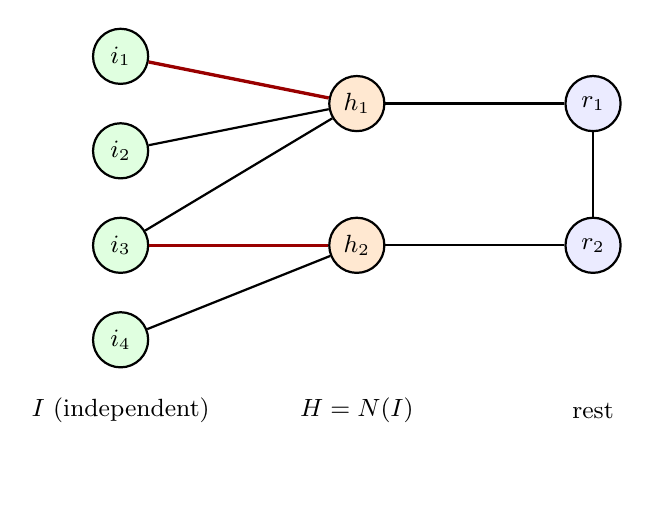
\begin{tikzpicture}[every node/.style={circle,draw,minimum size=7mm,inner sep=1pt,font=\small},thick]
  \begin{scope}[every node/.append style={fill=green!12}]
    \node (i1) at (0,2.4) {$i_1$};
    \node (i2) at (0,1.2) {$i_2$};
    \node (i3) at (0,0)   {$i_3$};
    \node (i4) at (0,-1.2){$i_4$};
  \end{scope}
  \begin{scope}[every node/.append style={fill=orange!18}]
    \node (h1) at (3,1.8) {$h_1$};
    \node (h2) at (3,0)   {$h_2$};
  \end{scope}
  \begin{scope}[every node/.append style={fill=blue!8}]
    \node (r1) at (6,1.8) {$r_1$};
    \node (r2) at (6,0)   {$r_2$};
  \end{scope}
  \draw[very thick,red!60!black] (h1)--(i1);
  \draw[very thick,red!60!black] (h2)--(i3);
  \draw (h1)--(i2);
  \draw (h2)--(i4);
  \draw (h1)--(i3);
  \draw (h1)--(r1);
  \draw (h2)--(r2);
  \draw (r1)--(r2);
  \node[draw=none,fill=none] at (0,-2.1) {$I$ (independent)};
  \node[draw=none,fill=none] at (3,-2.1) {$H=N(I)$};
  \node[draw=none,fill=none] at (6,-2.1) {rest};
\end{tikzpicture}
\caption{A crown $(I,H)$. The independent set $I$ on the left, its neighborhood $H$ in the middle, and a matching (thick red) that saturates $H$ into $I$. Every edge incident to $I$ must be covered; the saturating matching certifies that any cover needs at least $\abs{H}$ vertices for these edges, and taking all of $H$ achieves it.}
\label{ch25:fig-crown}
\end{figure}

\begin{focusbox}
\textbf{Crown reduction rule.} If $\Gph$ has a crown $(I,H)$, then there is a minimum vertex cover containing all of $H$ and none of $I$. Remove $I\cup H$ from $\Gph$ and set $k\gets k-\abs{H}$.
\end{focusbox}

\begin{whybox}
\textbf{Why it is safe.} The saturating matching $M$ pairs each $h\in H$ with a distinct $i\in I$. These $\abs{H}$ matching edges are vertex-disjoint, so \emph{any} cover must spend at least $\abs{H}$ vertices to cover them. Now compare two ways to cover all edges incident to $I$:
\begin{itemize}
  \item Take all of $H$: cost $\abs{H}$. Since $H=N(I)$, every edge touching $I$ has an endpoint in $H$, so this covers them all.
  \item Take some vertices of $I$ instead: the matching already forces $\ge \abs{H}$ vertices among $I\cup H$, and $I$ is independent, so $I$-vertices cover \emph{only} edges going to $H$ --- they buy you nothing outside the crown.
\end{itemize}
Hence given any cover $S$, the set $(S\setminus I)\cup H$ is a cover of size $\le\abs{S}$ by the matching lower bound. So an optimum cover taking all of $H$ and none of $I$ exists, and we may commit to it. \qed
\end{whybox}

How do we \emph{find} a crown? A clean route uses maximum matchings and the K\H{o}nig/Dulmage--Mendelsohn decomposition.

\begin{algorithm}[H]
\caption{\textsc{FindCrown}$(\Gph)$ --- crown via two matchings}
\label{ch25:alg-crown}
\DontPrintSemicolon
\KwIn{graph $\Gph=(V,E)$}
\KwOut{a crown $(I,H)$, or report ``no crown found''}
$M_1 \gets$ a maximum matching of $\Gph$\;
\lIf{$M_1$ saturates $V$}{ \Return ``no crown'' }
$O \gets$ set of $M_1$-unmatched vertices\;
$M_2 \gets$ a maximum matching of the bipartite graph between $O$ and $N(O)$\;
$H \gets$ vertices of $N(O)$ matched by $M_2$\;
$I \gets$ vertices reachable from $O$ by $M_2$-alternating paths, restricted to the $O$-side\;
\Return $(I,H)$\;
\end{algorithm}

The construction guarantees that whenever $\Gph$ has more than $3k$ vertices after Buss, a crown exists and is found, driving the kernel to at most $3k$ vertices.

\begin{theorem}[Linear crown kernel]\label{ch25:thm-crown-kernel}
Exhaustively applying Buss's rules and the crown reduction yields, in polynomial time, an equivalent vertex-cover instance with at most $3k$ vertices, or correctly reports \textsc{No}.
\end{theorem}

\begin{connectionbox}
The strongest known vertex-cover kernel comes not from crowns but from \emph{linear programming}. Relax the integer program to $x_v\in[0,1]$ with $x_u+x_v\ge 1$ per edge; by the Nemhauser--Trotter theorem the LP has a half-integral optimum $x_v\in\{0,\tfrac12,1\}$, and there is an optimum integral cover taking every $v$ with $x_v=1$ and no $v$ with $x_v=0$. Removing those decided vertices leaves only the all-$\tfrac12$ core, of size $\le 2k$. The LP is solvable by a single bipartite matching (LP duality $=$ K\H{o}nig), so this $2k$ kernel is computable in near-linear time. The same half-integrality powers the ``above-LP'' FPT algorithm of Lokshtanov, Narayanaswamy, Raman, Ramanujan and Saurabh. This is the polyhedral viewpoint of the companion linear-algebra book paying off: the geometry of the LP polytope hands you the kernel.
\end{connectionbox}

\begin{complexitybox}
\textbf{Vertex cover, the parameterized scorecard.}
\begin{center}
\begin{tabular}{lll}
\toprule
Technique & Result & Cost \\
\midrule
Naive enumeration & XP & $\Oh(n^k)$ \\
Bounded search tree & FPT & $\Oh(2^k(n+m))$ \\
Refined branching & FPT & $\Oh(1.466^k\,\poly)$, best $\approx 1.2^k$ \\
Buss kernel & quadratic & $\Oh(k^2)$ vertices/edges \\
Crown kernel & linear & $\le 3k$ vertices \\
LP / Nemhauser--Trotter kernel & linear & $\le 2k$ vertices \\
\bottomrule
\end{tabular}
\end{center}
Best practice: kernelize to $2k$ vertices, \emph{then} branch on the kernel. The branching cost becomes $\Oh(1.2^k\cdot k^{O(1)})$ with no $n$ anywhere near the exponent.
\end{complexitybox}

\section{Iterative compression: feedback vertex set}

The third technique answers a recurring difficulty: many problems are easy to \emph{verify and shrink} a candidate solution but hard to build one from scratch. \emph{Iterative compression}, introduced by Reed, Smith and Vetta for odd cycle transversal, turns ``I have a solution of size $k+1$, find one of size $k$'' into the engine of an FPT algorithm. We use it on \textsc{Feedback Vertex Set} (FVS): find $\le k$ vertices whose deletion makes the graph a forest (acyclic).

\subsection{The compression scaffold}

Build the graph up one vertex at a time. Maintain the invariant: \emph{after processing the first $i$ vertices, we hold a feedback vertex set $S_i$ of size $\le k$ for the induced subgraph $\Gph_i$}. Add the next vertex $v_{i+1}$. Then $S_i\cup\{v_{i+1}\}$ is an FVS of $\Gph_{i+1}$ of size $\le k+1$ (adding a vertex to an FVS keeps it an FVS). Now run a \emph{compression} routine: given an FVS of size $k+1$, either produce one of size $\le k$, or prove none exists --- in which case the whole instance is a \textsc{No}.

\begin{algorithm}[H]
\caption{\textsc{IterativeFVS}$(\Gph,k)$ --- build-and-compress}
\label{ch25:alg-itercomp}
\DontPrintSemicolon
\KwIn{graph $\Gph=(V,E)$ with $V=\{v_1,\dots,v_n\}$, budget $k$}
\KwOut{an FVS of size $\le k$, or \textsc{None}}
$S \gets \emptyset$;\quad $V_0\gets\emptyset$\;
\For{$i\gets 1$ \KwTo $n$}{
  $V_i\gets V_{i-1}\cup\{v_i\}$;\quad $\Gph_i\gets \Gph[V_i]$\;
  $W \gets S\cup\{v_i\}$ \tcp*{FVS of $\Gph_i$ of size $\le k+1$}
  $S \gets \textsc{Compress}(\Gph_i, W, k)$\;
  \lIf{$S = \textsc{None}$}{ \Return \textsc{None} }
}
\Return $S$\;
\end{algorithm}

The outer loop runs $n$ times; if each \textsc{Compress} call is FPT in $k$, the whole thing is FPT.

\subsection{The compression step}

We are given an FVS $W$ with $\abs{W}=k+1$ and want a smaller one. The trick is to guess the \emph{intersection} of the new solution with the old one. Iterate over all subsets $Z\subseteq W$ that the new solution $S$ keeps (so $Z = S\cap W$); there are $2^{k+1}$ of them. Vertices in $W\setminus Z$ are then \emph{forbidden} from $S$. After committing $Z$ to the solution and deleting it, we must find an FVS of size $\le k-\abs{Z}$ in the remaining graph that uses \emph{no} vertex of $W\setminus Z$. This is the \emph{disjoint compression} problem:

\begin{quote}
\textsc{Disjoint-FVS}: given $\Gph$ and a feedback vertex set $W'$ (here $W\setminus Z$) such that $\Gph - W'$ is a forest, find an FVS of size $\le k'$ that is \emph{disjoint} from $W'$.
\end{quote}

\begin{whybox}
Why is \textsc{Disjoint-FVS} easier? Because the forbidden set $W'$ induces a forest \emph{and} $\Gph - W'$ is a forest. So $\Gph$ is the union of two forests plus the edges between them --- a highly constrained structure. The solution we seek lives entirely in the forest $F=\Gph-W'$, and we must break every cycle of $\Gph$ that survives when we are not allowed to touch $W'$. A vertex of $F$ with $\ge 2$ edges into $W'$, or one lying on a path between two $W'$-vertices through $F$, is a pressure point. A small further branching --- repeatedly take a leaf of $F$ into the solution or push it to the $W'$-side --- solves \textsc{Disjoint-FVS} in $\Oh(c_0^{k}\poly)$, and modern analyses reach $\Oh(4^{k}\poly)$ or better.
\end{whybox}

\begin{algorithm}[H]
\caption{\textsc{Compress}$(\Gph,W,k)$ --- shrink an FVS by guessing its overlap}
\label{ch25:alg-compress}
\DontPrintSemicolon
\KwIn{graph $\Gph$, FVS $W$ with $\abs{W}=k+1$, budget $k$}
\KwOut{an FVS of size $\le k$, or \textsc{None}}
\For{each subset $Z\subseteq W$ with $\abs{Z}\le k$}{
  $W'\gets W\setminus Z$ \tcp*{kept from old solution; forbidden for new}
  \If{$\Gph[W']$ is acyclic}{
    $R \gets \textsc{DisjointFVS}(\Gph - Z,\; W',\; k-\abs{Z})$\;
    \lIf{$R\neq\textsc{None}$}{ \Return $Z\cup R$ }
  }
}
\Return \textsc{None}\;
\end{algorithm}

\begin{whybox}
\textbf{Correctness of compression.} Suppose $\Gph_i$ has an FVS $S^\star$ of size $\le k$. Let $Z^\star = S^\star\cap W$. The loop eventually tries $Z=Z^\star$. Then $W' = W\setminus Z^\star$ consists of old-solution vertices not reused; since $S^\star\cap W' = \emptyset$, the set $S^\star\setminus Z^\star$ is an FVS of $\Gph - Z^\star$ disjoint from $W'$ of size $\le k-\abs{Z^\star}$ --- exactly what \textsc{DisjointFVS} searches for, and finds. Conversely any $Z\cup R$ returned is an FVS of size $\le k$ by construction. The guard ``$\Gph[W']$ acyclic'' is needed because the disjoint subproblem assumes the forbidden set induces a forest; if it does not, no disjoint solution exists for that $Z$ and we skip it.
\end{whybox}

\begin{complexitybox}
\textsc{Compress} tries $2^{k+1}$ subsets $Z$; each calls \textsc{DisjointFVS}, FPT in $k$ at cost $\Oh(c_0^{k}\poly)$. So one compression costs $\Oh(2^{k+1}c_0^{k}\poly)=\Oh(c^k\poly)$ for a constant $c$. The outer loop multiplies by $n$. Total \textsc{IterativeFVS}: $\Oh(c^{k}\cdot n\cdot\poly)$, fixed-parameter tractable. The classical bound from this scaffold is around $\Oh(5^k\cdot kn)$; refined branchings reach $\Oh(3.46^k)$ and randomized methods $\Oh(3^k)$.
\end{complexitybox}

\subsection{Trace iterative compression on the running graph}

Take $\Gph$ from Figure~\ref{ch25:fig-running} with $k=2$. Its short cycles are the triangles $a\,b\,d$, $b\,c\,d$, $c\,d\,e$ and the $4$-cycle $c\,e\,f\,g$. Vertex $d$ sits on the first three; the fourth avoids $d$ entirely, which is what forces the second solution vertex.

\begin{labbox}
Add vertices in order $a,b,c,d,e,f,g$.
\begin{itemize}
  \item After $a,b$: only edge $ab$, no cycle. $S=\emptyset$.
  \item Add $c$: edges $ab,bc$. Still a tree. $S=\emptyset$.
  \item Add $d$: two triangles appear at once, $a\,b\,d$ (edges $ab,ad,bd$) and $b\,c\,d$ (edges $bc,bd,cd$), sharing the edge $bd$. $W=\{d\}$, size $1\le k+1$. Compress with budget $2$: $d$ lies on both triangles, so $\{d\}$ breaks both and has size $1\le 2$. $S=\{d\}$.
  \item Add $e$: triangle $c\,d\,e$ appears. Does $\{d\}$ still work? Deleting $d$ kills $abd$, $bcd$ and $cde$ at once. Yes. $S=\{d\}$.
  \item Add $f$: edge $ef$, $f$ a leaf, no new cycle. $S=\{d\}$.
  \item Add $g$: edges $cg,fg$, the $4$-cycle $c\,e\,f\,g$ appears and does \emph{not} contain $d$. So $\{d\}$ fails. Set $W=\{d,g\}$ (size $2\le k+1$). Compress with budget $2$: $\{d,g\}$ hits $abd$ (d), $bcd$ (d), $cde$ (d), $cefg$ (g) --- all cycles broken, size $2\le k$. $S=\{d,g\}$.
\end{itemize}
So $\Gph$ has an FVS of size $2$, e.g.\ $\{d,g\}$. This is in fact optimal: no single vertex breaks every cycle, because triangle $a\,b\,d$ and the $4$-cycle $c\,e\,f\,g$ are vertex-disjoint, so any FVS needs at least one vertex from each, hence size $\ge 2$. (A tempting guess is $\{c\}$, since $c$ lies on $bcd$, $cde$ and $cefg$; but $c$ misses triangle $abd$, so $\{c\}$ leaves the cycle $a\,b\,d$ intact.) Iterative compression certifies \emph{a} solution of size $\le k$ for the $k$ you ask for; to get the minimum, run it with the target $k$ (or binary-search $k$ upward).
\end{labbox}

\section{Color coding: the longest path}

The fourth technique is the cleverest. \textsc{Longest Path} (does $\Gph$ contain a simple path on $k$ vertices?) is NP-hard for general $k$, and the obstacle is the word ``simple'': a walk of length $k$ is trivial by matrix powering, but forbidding repeated vertices is what makes it hard. \emph{Color coding}, due to Alon, Yuster and Zwick, sidesteps the repetition problem with randomness: color the vertices with $k$ colors at random and look only for \emph{colorful} paths --- paths using each color exactly once. A colorful path is automatically simple, and colorfulness is exactly what dynamic programming over color \emph{subsets} can track.

\begin{intuitionbox}
Searching for a simple $k$-path directly forces you to remember which vertices you have used --- a set of up to $n$ possibilities, exponential. Random coloring replaces ``which vertices'' with ``which colors,'' and there are only $k$ colors, so the bookkeeping set has $2^k$ states instead of $2^n$. The price is randomness: a fixed $k$-path becomes colorful only some of the time. But the probability is good enough, $k!/k^k\approx e^{-k}$, that $\Oh(e^k)$ independent colorings catch it with high probability. We pay $e^k$ to demote the exponent from $n$ to $k$.
\end{intuitionbox}

\subsection{Colorful-path dynamic programming}

Color each vertex with a uniformly random color in $\{1,\dots,k\}$. A path is \emph{colorful} if its $k$ vertices carry $k$ distinct colors. We seek a colorful path on $k$ vertices. Dynamic program: for each vertex $v$ and each color set $C\subseteq\{1,\dots,k\}$, let
\[
  D[v,C] = \text{true} \iff \text{there is a colorful path ending at }v\text{ using exactly the color set }C.
\]
Then $D[v,\{\mathrm{color}(v)\}]=\text{true}$ for every $v$, and
\[
  D[v,C] = \bigvee_{\substack{u\sim v\\ \mathrm{color}(v)\in C}}\; D[u,\; C\setminus\{\mathrm{color}(v)\}].
\]
A colorful $k$-path exists iff $D[v,\{1,\dots,k\}]=\text{true}$ for some $v$.

\begin{algorithm}[H]
\caption{\textsc{ColorfulPath}$(\Gph,k,\mathrm{color})$ --- DP over color subsets}
\label{ch25:alg-colorcoding}
\DontPrintSemicolon
\KwIn{graph $\Gph=(V,E)$, target length $k$, a coloring $\mathrm{color}:V\to\{1,\dots,k\}$}
\KwOut{\textsc{True} if a colorful $k$-path exists under this coloring}
\lForEach{$v\in V$}{ set $D[v,\{\mathrm{color}(v)\}]\gets\textsc{True}$, all other $D[v,\cdot]\gets\textsc{False}$ }
\For{$s\gets 2$ \KwTo $k$}{
  \ForEach{color set $C$ with $\abs{C}=s$}{
    \ForEach{$v$ with $\mathrm{color}(v)\in C$}{
      \ForEach{neighbor $u\sim v$}{
        \lIf{$D[u,\;C\setminus\{\mathrm{color}(v)\}]$}{ set $D[v,C]\gets\textsc{True}$ }
      }
    }
  }
}
\Return $\bigvee_{v} D[v,\{1,\dots,k\}]$\;
\end{algorithm}

\begin{whybox}
\textbf{Correctness of the DP.} Induction on path length $s$. Base $s=1$: the single-vertex path at $v$ uses color set $\{\mathrm{color}(v)\}$. Step: a colorful path of $s$ vertices ending at $v$ with color set $C$ is a colorful path of $s-1$ vertices ending at some neighbor $u$ with color set $C\setminus\{\mathrm{color}(v)\}$, extended by the edge $uv$ --- and $\mathrm{color}(v)$ must lie in $C$ but not in the prefix's set, which is precisely the recurrence. Colorfulness is enforced because $C$ is a \emph{set}: re-using a color cannot grow $\abs{C}$, so a path that revisits a color never reaches $\abs{C}=s$. A colorful path is simple because distinct colors force distinct vertices. \qed
\end{whybox}

\begin{whybox}
\textbf{Success probability.} Fix any simple $k$-path $P$ in $\Gph$ (if one exists). Under a uniform random coloring, the $k$ vertices of $P$ get $k$ distinct colors with probability
\[
  \Pr[P\text{ colorful}] = \frac{k!}{k^k} \ge \frac{\sqrt{2\pi k}\,(k/e)^k}{k^k} = e^{-k}\sqrt{2\pi k}\;\ge\; e^{-k},
\]
using Stirling. So one random coloring detects a fixed target path with probability $\ge e^{-k}$. Repeating with $N = \lceil e^k\rceil$ independent colorings, the chance of missing $P$ in \emph{all} of them is $\le (1-e^{-k})^{e^k}\le e^{-1}$. Taking $N = \lceil c\cdot e^k\rceil$ colorings drops the failure probability to $e^{-c}$, as small as we like. The algorithm has one-sided error: it never reports a path that is not there (the DP only finds genuine colorful, hence simple, paths), and it finds an existing path with probability $\ge 1-e^{-c}$.
\end{whybox}

\begin{complexitybox}
One DP pass fills a table of $\Oh(2^k\cdot n)$ entries, each touching $\Oh(\deg)$ neighbors, for $\Oh(2^k\cdot m)$ time. Repeating $\Oh(e^k)$ times for high probability gives
\[
  \Oh\!\big((2e)^k\cdot m\cdot \log(1/\delta)\big) = 2^{O(k)}\cdot m,
\]
fixed-parameter tractable in $k$, with failure probability $\delta$. Derandomization via \emph{$(n,k)$-perfect hash families} replaces the random colorings by a deterministic family of $\Oh(e^k k^{O(\log k)}\log n)$ colorings guaranteed to make any fixed $k$-set colorful at least once, yielding a deterministic $2^{O(k)}\poly(n)$ algorithm. The algebraic descendant of Koutis and Williams pushes the base to $2^k$.
\end{complexitybox}

\subsection{Trace color coding by hand}

Look for a path on $k=4$ vertices in $\Gph$ (Figure~\ref{ch25:fig-running}). A real one exists, e.g.\ $a\,b\,c\,g$.

\begin{labbox}
Pick the coloring $\mathrm{color}(a)=1,\ b=2,\ c=3,\ d=1,\ e=4,\ f=3,\ g=4$. Hunt for a colorful $4$-path (colors $\{1,2,3,4\}$ all distinct).
\begin{itemize}
  \item Length $1$: $D[a,\{1\}],D[b,\{2\}],D[c,\{3\}],D[d,\{1\}],D[e,\{4\}],D[f,\{3\}],D[g,\{4\}]$ all true.
  \item Length $2$: edge $a\,b$ gives $D[b,\{1,2\}]$; edge $b\,c$ gives $D[c,\{2,3\}]$; edge $c\,g$ gives $D[g,\{3,4\}]$; edge $d\,e$ gives $D[e,\{1,4\}]$.
  \item Length $3$: extend $D[b,\{1,2\}]$ along $b\,c$ ($\mathrm{color}(c)=3$): $D[c,\{1,2,3\}]$ true (path $a\,b\,c$). Extend $D[c,\{2,3\}]$ along $c\,g$: $D[g,\{2,3,4\}]$ true (path $b\,c\,g$).
  \item Length $4$: extend $D[c,\{1,2,3\}]$ (path $a\,b\,c$) along $c\,g$, $\mathrm{color}(g)=4$: $D[g,\{1,2,3,4\}]$ true. Colorful $4$-path found: $a\,b\,c\,g$ with colors $1,2,3,4$.
\end{itemize}
This coloring happened to make $a\,b\,c\,g$ colorful, so one pass succeeded. With $k=4$ the per-path success chance is $4!/4^4 = 24/256 \approx 0.094$, so about $11$ colorings suffice on average to hit a given path; had this one failed we would simply re-roll.
\end{labbox}

\begin{applicationbox}
Color coding is the workhorse for \emph{subgraph counting} in biological networks. To estimate how often a small motif (a $k$-vertex pattern, like a feed-forward loop) occurs in a protein-interaction or gene-regulatory graph, color the host graph and count colorful occurrences of the motif by exactly this subset DP; an unbiased estimator divides by the colorful probability. It also underlies FPT algorithms for \textsc{$k$-Path}, \textsc{Tree Subgraph Isomorphism} and \textsc{Graph Motif}, and its algebraic descendant --- replacing colors by random field elements and detecting a multilinear monomial via a determinant over a polynomial ring (Koutis--Williams) --- gives the $\Oh(2^k)$ longest-path algorithm that beats naive color coding.
\end{applicationbox}

\section{When nothing works: the W-hierarchy}

Four techniques, four FPT victories. But some parameterized problems stubbornly resist all of them. \textsc{Clique} (is there a clique of size $k$?) and \textsc{Dominating Set} (is there a dominating set of size $k$?) have no known $f(k)\cdot\poly(n)$ algorithm, and the best anyone has is the XP brute force $\Oh(n^k)$. We would like a hardness theory explaining why --- a parameterized analogue of NP-completeness.

\begin{intuitionbox}
NP-completeness rests on polynomial-time reductions and a complete problem (SAT). Parameterized hardness rests on \emph{FPT reductions} --- reductions that run in FPT time and map parameter $k$ to a new parameter $k'\le g(k)$ bounded by a function of $k$ only --- and a hierarchy of increasingly hard problems indexed by the ``depth'' of the circuits needed to verify a solution. That hierarchy is the W-hierarchy:
\[
  \mathrm{FPT}\subseteq \mathrm{W[1]}\subseteq \mathrm{W[2]}\subseteq\cdots\subseteq \mathrm{W[P]}\subseteq \mathrm{XP}.
\]
Each containment is conjectured strict. W[1] is the parameterized world's NP: ``W[1]-hard'' is the verdict ``almost certainly not FPT.''
\end{intuitionbox}

\begin{definition}[FPT reduction]\label{ch25:def-fptred}
An \emph{FPT reduction} from $(A,\kappa_A)$ to $(B,\kappa_B)$ maps an instance $(x,k)$ to an instance $(x',k')$ such that: (i) $(x,k)\in A \iff (x',k')\in B$; (ii) the map runs in time $f(k)\cdot\abs{x}^{O(1)}$; (iii) $k'\le g(k)$ for some computable $g$. If $A$ FPT-reduces to $B$ and $B\in\mathrm{FPT}$, then $A\in\mathrm{FPT}$.
\end{definition}

\begin{whybox}
Why must $k'$ stay bounded by $g(k)$? Because if a reduction were allowed to inflate the parameter to, say, $k'=n$, then an $f(k')\poly$ algorithm for $B$ would cost $f(n)\poly$ on $A$ --- not FPT at all. The parameter is the resource being tracked, and FPT reductions must not smuggle hardness from $n$ into $k'$. This is the single discipline that makes the whole theory coherent, and it is exactly the same discipline as the kernel definition's ``$k'\le k$.''
\end{whybox}

The hierarchy is defined via weighted circuit satisfiability. \textsc{Weighted Circuit-SAT}: given a Boolean circuit $C$ and integer $k$, is there an input of \emph{weight} exactly $k$ (exactly $k$ ones) that satisfies $C$? Parameterizing by $k$ and restricting the \emph{weft} (the number of large-fan-in gates on any input-to-output path) to $t$ defines W[$t$].

\begin{focusbox}
\textbf{Canonical complete problems.}
\begin{itemize}
  \item \textsc{Independent Set} and \textsc{Clique} are W[1]-complete (under FPT reductions). They are the ``parameterized SAT'' of the field: a problem is ``probably not FPT'' precisely when it is W[1]-hard.
  \item \textsc{Dominating Set} is W[2]-complete --- one level harder, reflecting the extra alternation in ``every vertex is dominated.''
  \item \textsc{Vertex Cover}, \textsc{FVS}, \textsc{Longest Path} are in FPT (this chapter), the easy end of the spectrum.
\end{itemize}
\end{focusbox}

\begin{whybox}
\textbf{Why \textsc{Clique} is believed not FPT.} Suppose \textsc{Clique} parameterized by $k$ were FPT, solvable in $f(k)n^c$. The \emph{Exponential Time Hypothesis} (ETH) of Impagliazzo and Paturi posits that $3$-SAT on $n$ variables cannot be solved in $2^{o(n)}$ time. A classical chain of reductions shows that even an $n^{o(k)}$ algorithm for \textsc{Clique} would yield a $2^{o(n)}$ algorithm for $3$-SAT, contradicting ETH. So under ETH, \textsc{Clique} has no $n^{o(k)}$ algorithm, let alone an FPT one; the brute-force $\Oh(n^k)$ is essentially optimal. W[1]-hardness packages this kind of evidence into a reusable certificate: prove your problem W[1]-hard and you have shown it is, modulo widely-believed conjectures, not FPT.
\end{whybox}

\begin{trapbox}
A frequent confusion: ``W[1]-hard'' does not mean ``not in XP.'' \textsc{Clique} \emph{is} in XP (the $n^k$ brute force). W[1]-hardness is a statement about the \emph{exponent's location}: the $k$ refuses to come off $n$. Likewise, ``FPT'' does not mean ``practical'' --- a $2^{2^k}n$ algorithm is FPT and hopeless for $k=6$. And the parameter is a modeling choice: \textsc{Dominating Set} is W[2]-hard parameterized by solution size but FPT parameterized by treewidth. Always state the parameter before claiming hardness or tractability.
\end{trapbox}

\begin{connectionbox}
The treewidth chapter (Chapter~24) and this one are two halves of one story. Courcelle's theorem says every problem expressible in monadic second-order logic is FPT parameterized by treewidth --- a single meta-theorem subsuming vertex cover, FVS, dominating set, $3$-coloring and hundreds more, all FPT \emph{when the graph is tree-like}. The bounded-search-tree and color-coding results here parameterize by \emph{solution size} instead, a different knob that works on arbitrary graphs. Together: parameterize by structure (treewidth, planarity, genus) or by solution size, and a huge swath of NP-hard graph problems becomes tractable. The W-hierarchy marks the boundary where neither knob is known to help.
\end{connectionbox}

\section*{Summary}

\begin{center}
\begin{tabular}{lll}
\toprule
Technique & Idea & Flagship result \\
\midrule
Bounded search tree & branch, shrink $k$ each branch & VC in $\Oh(2^k(n+m))$ \\
Kernelization & poly-time shrink to size $g(k)$ & VC kernel $\le 2k$ vertices \\
Iterative compression & build up, compress $k{+}1\!\to\!k$ & FVS in $\Oh(c^k\,kn)$ \\
Color coding & random colors make paths simple & $k$-Path in $2^{O(k)}m$ \\
W-hierarchy & FPT reductions, weft levels & Clique W[1]-hard \\
\bottomrule
\end{tabular}
\end{center}

The thread running through all four: find the parameter that captures the hardness, then engineer the exponential dependence to touch only that parameter. When you can, you get FPT. When you provably cannot (W[1]-hardness, under ETH), you have learned something equally valuable --- that the parameter you chose is the wrong knob, and you should go looking for another.

\begin{connectionbox}
\textbf{What This Unlocked:}
Parameterized complexity rescued dozens of NP-hard problems from theoretical paralysis.
By quarantining exponential growth to an auxiliary parameter $k$, algorithms like bounded
search trees, kernelization (Buss and Crown rules), iterative compression, and color
coding run in polynomial time for small $k$ on massive graphs ($n \ge 10^6$). Kernelization
provides a mathematically rigorous foundation for data reduction and preprocessing pipelines.

\textbf{Honest Downsides and Limitations:}
\begin{itemize}
  \item \emph{Small parameters only:} FPT algorithms are practical only when $k$ is small
        (typically $k \le 20\text{--}40$). When $k = \Om(n)$ or $k = \Om(\log n)$ with
        superexponential $f(k)$, the running time degenerates into brute force.
  \item \emph{W-hardness barriers:} Many critical problems ($k$-Clique, $k$-Independent Set,
        $k$-Dominating Set) are $W[1]$- or $W[2]$-hard, provably precluding $f(k)\cdot n^{\Oh(1)}$
        algorithms under standard complexity conjectures (like the Exponential Time Hypothesis).
  \item \emph{Non-polynomial kernels:} Many FPT problems admit kernels of exponential size
        $2^{\Oh(k)}$ but provably have no polynomial-size kernel unless $\mathrm{NP} \subseteq \mathrm{coNP/poly}$.
\end{itemize}

\textbf{Where We Go Next:}
When parameterization by solution size fails on general graphs, geometric and topological
constraints can come to our rescue. If a graph can be drawn in the plane without crossing edges,
topological properties dramatically restrict its structure. In \textbf{Chapter~26 (Planar Graphs
and Planarity Testing)}, we explore Euler's formula $V - E + F = 2$ and Kuratowski's theorem,
which lay the groundwork for bidimensionality theory and subexponential $2^{\Oh(\sqrt{k})}\cdot n$
algorithms on planar graphs.
\end{connectionbox}

\section{Exercises}

\begin{exercise}[Refined VC branching]
Prove that the branching rule ``pick a vertex $v$ of degree $\ge 3$; branch (a) $v\in S$, recurse on $\Gph-v$ with $k-1$, or (b) $v\notin S$, put all of $N(v)$ in $S$, recurse on $\Gph-v-N(v)$ with $k-\deg(v)$'' has running time $\Oh(1.466^k\poly)$ once degree-$\le 2$ vertices are eliminated by reduction. Solve the recurrence $T(k)=T(k-1)+T(k-3)$ and identify the characteristic root.
\end{exercise}

\begin{exercise}[Buss kernel by hand]
Run Buss's reduction on the graph of Figure~\ref{ch25:fig-running} with $k=4$. Which vertices (if any) are forced by Rule~2? What is the resulting kernel, and does the ``$>k^2$ edges'' rule fire? Conclude whether a size-$4$ cover exists.
\end{exercise}

\begin{exercise}[Crown correctness, sharpened]
Prove that if $(I,H)$ is a crown then \emph{every} minimum vertex cover that takes some vertex of $I$ can be transformed into one of equal size taking all of $H$ and none of $I$. Where exactly does the saturating matching get used in your argument?
\end{exercise}

\begin{exercise}[No crown, no shrink]
Construct a graph on which Buss's rules and the crown reduction both fail to reduce the instance below $2k$ vertices for some $k$, yet the LP/Nemhauser--Trotter kernel still shrinks it. (Hint: a graph whose LP optimum is all-$\tfrac12$.)
\end{exercise}

\begin{exercise}[Iterative compression for OCT]
Adapt the iterative-compression scaffold to \textsc{Odd Cycle Transversal}: delete $\le k$ vertices to make the graph bipartite. Describe the disjoint-compression subproblem and explain why it reduces to a sequence of min-cut / max-flow computations. (This is the original Reed--Smith--Vetta result.)
\end{exercise}

\begin{exercise}[Why colorful equals simple]
Prove carefully that in the color-coding DP, every path counted by $D[v,C]$ with $\abs{C}=s$ visits $s$ distinct vertices. Then exhibit a (non-colorful) coloring under which a real simple $k$-path is missed, and compute the probability of that miss for $k=5$.
\end{exercise}

\begin{exercise}[Derandomizing color coding]
State the definition of an $(n,k)$-perfect hash family and show that, given such a family of size $N(n,k)$, the randomized color-coding algorithm becomes deterministic at a multiplicative cost of $N(n,k)$. Look up the best known bound on $N(n,k)$ and write down the resulting deterministic running time for \textsc{$k$-Path}.
\end{exercise}

\begin{exercise}[FPT reductions preserve FPT]
Prove Definition~\ref{ch25:def-fptred}'s closure claim: if $A$ FPT-reduces to $B$ and $B\in\mathrm{FPT}$, then $A\in\mathrm{FPT}$. Where in the argument do you use $k'\le g(k)$? Show by example that dropping this condition breaks the implication.
\end{exercise}

\begin{exercise}[Clique and independent set]
Give an FPT reduction from \textsc{Independent Set} (parameter $k$) to \textsc{Clique} (parameter $k$) and back, using the complement graph. Why does this show the two are equivalent under FPT reductions, and why does it \emph{not} by itself prove either is W[1]-hard?
\end{exercise}

\begin{exercise}[Parameter matters]
\textsc{Dominating Set} is W[2]-hard parameterized by solution size. Show it is FPT parameterized by treewidth by sketching a DP over a tree decomposition with states recording, for each bag vertex, whether it is in the set / dominated / not-yet-dominated. What is the dependence on treewidth $w$? (Expect $\Oh(3^w\cdot\poly)$ or so.)
\end{exercise}

\begin{exercise}[Break the budget bug]
Take the buggy branching from the Common-trap box (``$u\notin S$, recurse with $k$ unchanged''). Construct a small graph and budget $k$ on which this buggy algorithm either over-explores without terminating in the claimed bound or returns a wrong answer, and explain precisely which invariant it violates.
\end{exercise}
